Dust impacts happen randomly, and are uncorrelated with each other, fulfilling the~definition of {Poisson point process} (PPP). Since detections might be relatively rare, the~fitting routine must be chosen and carried out carefully to yield the~available information. Several approaches are commonly taken and in this chapter, the~most important and commonly used ones are introduced, demonstrated and practically compared. As we will see, not all of the~common algorithms are always appropriate. Notably, the~least squares fitting is problematic for Poisson process, and more appropriate algorithms are introduced in this chapter.

\section{Poisson point process}

The~defining feature of PPP is that it consists of points $\vec{\omega}$ located randomly and independently of each other in the~mathematical space of interest $\Omega$. This space might be the~physical space $\Omega_{3D}$ with the~process modelling locations of events, or $\Omega$ might be the~timeline $\Omega_{time}$, and then PPP models \textit{when} events happen. In the~case of in-situ detection of cosmic dust, the~space is the~physical space $\Omega_{3D}$, but since the~location of the~spacecraft is implicitly bound with time through its trajectory, the~problem is usually solved on the~timeline $\Omega_{time}$.

Let $A$ be a~subset of $\Omega$. a~feature of PPP is that the~number of points $N$ within $A$ is a~random variable, which follows the~\textit{Poisson distribution} with the~probability mass function:
\begin{equation}
    P(N=n) = \mathrm{Pois}(n,\Lambda) \equiv \frac{\Lambda^n e^{-\Lambda}}{n!}, \label{eq:poisson_pmf}
\end{equation}
where $\Lambda = \mathbb{E}(N)$ is the~expected value of $N$. In the~special case of \textit{homogeneous} PPP, $\Lambda$ is proportional to the~\textit{measure} $\mu$ of $A$ in $\Omega$ with the~scaling factor of $\lambda$:
\begin{equation}
    \Lambda = \lambda \mu(A),
\end{equation}
where $\lambda$ is called the~\textit{rate}. In the~general case of PPP, $\lambda$ is a~non-negative function of the~location $\omega$ in $\Omega$:
\begin{equation}
    \lambda = \lambda(\omega) \geq 0; \ \omega \in \Omega,
\end{equation}
and then 
\begin{equation}
    \Lambda = \int_A \lambda(\omega) \, d\mu.
\end{equation}
In the~special case of $\Omega$ being the~timeline $\Omega_{time}$, and $A$ being the~interval of observation between the~times $t_{start}$ and $t_{stop}$, we have
\begin{equation}
    \Lambda = \int_{t_{start}}^{t_{stop}} \lambda(t) \, dt.
\end{equation}
This is an appropriate model for the~number of dust detections $N$ detected over a~temporal interval $(t_{start},t_{stop})$.

\section{Maximum likelihood estimation} \label{ch:mle}

Assume the~following experimental scheme: let \textit{data} $\vec{x} = (x_1, x_2, \dots , x_k)$ be the~\textit{realizations} of a~random variable $X$, and let the~parametric probability density function (also called the~\textit{family}) of the~process $f_X$ be known, with the~\textit{parameters} $\vec{\theta}$ being unknown:
\begin{equation}
    f_X = f_X(x_i|\vec{\theta}). \label{eq:stat_experiment}
\end{equation}
This means that in a~repeated experiment, and given the~parameters $\vec{\theta}$, a~value $x_i$ is acquired with the~frequency proportional to $f_X(x_i|\vec{\theta})$. The~usual goal is to find the~underlying $\vec{\theta}$, which is the~most compatible with the~experiment results $\vec{x}$. \textit{Likelihood} $\mathcal{L}=\mathcal{L}(\vec{\theta})$ is a~function of $\vec{\theta}$ defined as 
\begin{equation}
    \mathcal{L}(\vec{\theta}|x_i) = f_X(x_i|\vec{\theta})
\end{equation}
in the~case of a~single data point $x_i$, where $|x_i$ means the~single data point $x_i$ is used to evaluate the~likelihood. The~intuitive meaning of likelihood is how well the~$\vec{\theta}$ corresponds to the~observed data point $x_i$. Since observing $x_i$ is more probable for $\vec{\theta}_1$ with high $\mathcal{L}(\vec{\theta}_1|x_i)$ than for $\vec{\theta}_2$ with low $\mathcal{L}(\vec{\theta}_2|x_i)$, one might say that $\vec{\theta}_1$ is more likely than $\vec{\theta}_2$, given $x_i$ was observed. We note that $\mathcal{L}$ is not a~probability distribution, since it is a~function of $\vec{\theta}$ rather than $\vec{x}$. Furthermore, it is generally not normalized, or even integrable. Should the~random vector $\vec{x}$ contain $k$ realizations of an independent random variable, the~likelihood of $\vec{\theta}$ given $\vec{x}$ is 
\begin{equation}
    \mathcal{L}(\vec{\theta}|\vec{x}) = \prod_{i=1}^k f_X(x_i|\vec{\theta}),
\end{equation}
where $\mathcal{L}$ retains all the~properties discussed earlier. Then maximum likelihood estimation is the~method of finding $\vec{\theta}_{max}$, which maximizes $\mathcal{L}$ in the~space $\Theta$ of possible $\vec{\theta}$. Such a~$\vec{\theta}_{max}$ is called the~\textit{maximum likelihood estiate} (MLE). We note that the~same $\vec{\theta}_{max}$ maximizes $\mathcal{L}(\vec{\theta}|\vec{x})$ and $l(\vec{\theta}|\vec{x}) = \log \left( \mathcal{L}(\vec{\theta}|\vec{x}) \right)$. Since 
\begin{equation}
    l(\vec{\theta}|\vec{x}) = \log \left( \mathcal{L}(\vec{\theta}|\vec{x}) \right) = \log \left( \prod_{i=1}^k f_X(x_i|\vec{\theta}) \right) =  \sum_{i=1}^k \log \left( f_X(x_i|\vec{\theta}) \right),
\end{equation}
the MLE is also found by maximizing $l$, so called \textit{log-likelihood}, which is often computationally much cheaper. 

In the~special case of $f_X$ being the~Poisson probability mass function (Eq.~\ref{eq:poisson_pmf}), there is a~single parameter $\Lambda$ to maximize $\mathcal{L}$ with. Having observed $k$ realizations (data points) $\vec{n} = (n_1, n_2, \dots , n_k)$, the~log-likelihood of $\Lambda$ is
\begin{equation}
    l(\Lambda|\vec{n}) = \sum_{i=1}^k \log \left( \frac{\Lambda^{n_k} e^{-\Lambda}}{n_k!} \right) = \log(\Lambda) \sum_{i=1}^k n_k - k \Lambda - \sum_{i=1}^k \log(n_k!),  
\end{equation}
where $\log(n!)$ is easily evaluated for small $n$ and can be cost-effectively very closely approximated for large $n$, using for example Ramanujan's approximation \citep{ramanujan1988lost}. 

It is also possible that the~rate $\Lambda$ was not constant during the~data acquisition, but changed with time $t$ as
\begin{equation}
    \Lambda = \Lambda(t,\vec{\xi}), \label{eq:compound_model}
\end{equation}
that is $\Lambda$ was a~parametric function of time $t$ with unknown parameters $\vec{\xi}$. If the~family $f_X$ is known, as is the~parametric function $\Lambda$, but not the~parameters $\vec{\xi}$, this might be solved the~same way, that is with maximizing (now more complicated) likelihood $\mathcal{L}$, or log-likelihood $l = \log(\mathcal{L})$. 

\section{Least squares estimation}

Assume experimental data $\vec{x}$ and unknown parameters vector $\vec{\theta}$. In addition, let us assume that $x_i$ of $\vec{x}$ are not independently distributed, but each $x_i$ has its own distribution function family $f_{X_i}$, which might for example represent a~time dependent experiment, such as the~one in Eq.~\ref{eq:compound_model}. Assuming a~value for the~parameters vector $\vec{{\theta}}$, a~vector of expected values of $\vec{\tilde{x}}(\vec{{\theta}}) = (\mathbb{E}(X_1|\vec{\theta}),\mathbb{E}(X_2|\vec{\theta}),\dots,\mathbb{E}(X_k|\vec{\theta}))$ is calculated. We evaluate $S$:
\begin{equation}
    S(\vec{{\theta}}) = || \vec{x} - \vec{\tilde{x}}(\vec{{\theta}}) ||_2 = \sum_{i=1}^{k} \left( x_i - \mathbb{E}(X_i|\vec{\theta}) \right)^2. \label{eq:least_squares}
\end{equation}
If the~parameter vector $\vec{{\theta}}$ minimizes $S$ in the~space of possible parameter vectors $\Theta$, then $\vec{{\theta}}$ is called the~\textit{least squares estiamte} (LSE). Weighted least squares estimate (WLSE) is a~modification of LSE, in which the~weights $w_i$ are introduced in Eq.~\ref{eq:least_squares}:
\begin{equation}
     S_w(\vec{{\theta}}) = \sum_{i=1}^{k} \left( w_i \left( x_i - \mathbb{E}(X_i|\vec{\theta}) \right) \right)^2, \label{eq:weighted_least_squares}
\end{equation}
where the~estimate is improved if the~weights are the~reciprocal standard deviations for each of the~data points $w_i = \sigma^{-1}$. Finding the~LSE is often computationally much cheaper than finding the~MLE as described in Sec.~\ref{ch:mle}, and in some special cases, they are equivalent. However, LSE is just a~mathematical optimization algorithom, which disregards the~distribution of the~data, and in general is not equivalent to MLE. 

\subsection{Maximum likelihood equivalence}

Assume: 
\begin{equation}
    f_{X_i}(x_i|\vec{\theta}) = \mathcal{N}(\mathbb{E}(X_i|\vec{\theta}),\sigma) = \frac{1}{\sqrt{2 \pi} \sigma} e^{-\left( \frac{x_i - \mathbb{E}(X_i|\vec{\theta})}{\sqrt{2} \sigma} \right)^2},
\end{equation}
that is, the~value observed in a~repeated experiment is \textit{normally distributed} around its expected value, or in other words, the~errors $\epsilon_i = x_i - \mathbb{E}(X_i|\vec{\theta})$ are \textit{Gaussian}. If independence of $\epsilon_i$ is assumed, then we get for log-likelihood:
\begin{equation}\begin{split}
    l(\vec{\theta}|\vec{x}) 
    &= \sum_{i=1}^{k} \log \left( f_{X_i}(x_i|\vec{\theta}) \right)  \\
    %&= \sum_{i=1}^{k} \log \left( \mathcal{N}(\mathbb{E}(X_i|\vec{\theta}),\sigma) \right) \\
    &= \sum_{i=1}^{k} \log \left( \frac{1}{\sqrt{2 \pi} \sigma} e^{-\left( \frac{x_i - \mathbb{E}(X_i|\vec{\theta})}{\sqrt{2} \sigma} \right)^2} \right) \\
    &= k\log\left(\frac{1}{\sqrt{2 \pi} \sigma}\right) - \frac{1}{2 \sigma^2} \sum_{i=1}^{k} \left(  x_i - \mathbb{E}(X_i|\vec{\theta}) \right)^2 \\
    &= k\log\left(\frac{1}{\sqrt{2 \pi} \sigma}\right) - \frac{S}{2 \sigma^2}, \label{eq:mle_lse_equivalence}
\end{split}\end{equation}
therefore by minimizing $S$, we maximized $l$ (compare Eqs.~\ref{eq:least_squares} and \ref{eq:mle_lse_equivalence}). We note we assumed a~single standard deviation $\sigma$ for all the~$x_i$, which might be generalized to individual $\sigma_i$ by weighting in the~sum (Eq.~\ref{eq:weighted_least_squares}). This can further be generalized for the~case of regular exponential family distributions \citep{charnes1976equivalence}, therefore also for Poisson distribution. In any case, we either evaluate or approximate MLE with LSE, which offers no advantages over the~straight evaluation of MLE beyond the~computational cost.

\subsection{Linear combination fitting}

A common experimental task is to explain an observed variable count as an unknown combination of known effects, which combine into a~rate. Let us have data $\vec{n} = (n_1, n_2, \dots , n_k)$, and assume
\begin{equation}
    f_{N_i}(n_i) = \mathrm{Pois}(n_i,\Lambda_i) = \mathrm{Pois}(n_i,\beta_1 \lambda_{1,i} + \beta_2 \lambda_{2,i} + \cdots + \beta_m \lambda_{m,i}), \label{eq:linear_comination_model}
\end{equation}
where unknown $\Lambda_i$ was not a~constant for all $i$, but was a~single unknown linear combination $\vec{\beta} = (\beta_1, \beta_2, \dots, \beta_m); \ \beta_i \geq 0 \ \forall i$ of known non-constant effects $\lambda_{1,i}, \lambda_{2,i}, \dots, \lambda_{m,i}$. This task is best approached keeping Poisson family in mind, which is not the~case when a~simple LSE of $\vec{\beta}$ is evaluated, which we show on an example. 

Comparing MLE and LSE for real experimental data is not very instructive, since the~true process is never really known. For this reason, we use a~toy model. Let us examine a~fit of such a~toy model, which retains the~most important characteristics of dust detection rate fitting. Assume we have observations $\vec{n}$ of a~Poisson-distributed random variable defined as
\begin{equation}
    f_{N_i}(n_i) = \mathrm{Pois}(n_i,\Lambda_i) = \mathrm{Pois}(n_i,\beta_1 y_i + \beta_2 y_i^5), \label{eq:toy_model}
\end{equation}
where $y_i$ are the~values of the~independent variable, so called \textit{covariate}, which produced the~actual rates $\Lambda_i$ according to
\begin{equation}
    \Lambda_i = \beta_1 y_i + \beta_2 y_i^5, \label{eq:toy_model_rate}
\end{equation}
which is a~linear combination of two polynomial terms. Let's further assume the~actual values of $\vec{\beta} = (\beta_1,\beta_2)$ are
\begin{equation}\begin{split}
    \beta_1 &= 1 \\
    \beta_2 &= 3, \label{eq:toy_beta_values}
\end{split}\end{equation}
and that we have a~set $\vec{n}$ of $150$ observations of $n_i$, which were drawn according to Eq.~\ref{eq:toy_model} with different covariates $y_i\in(0,2)$. One such a~draw is shown in Fig.~\ref{fig:toy_model_curve}. 

\begin{figure}[ht]
 	\centering
 	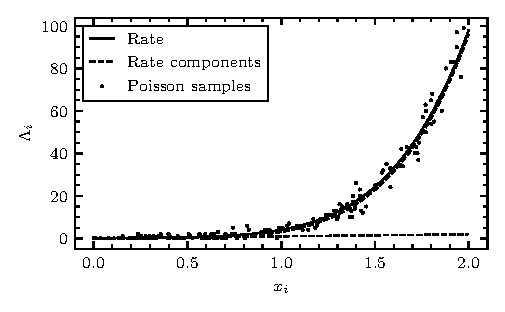
\includegraphics[width=10cm]{figures/toy_model_curve.pdf}
 	\caption{A possible realization of the~experiment defined by Eqs.~\ref{eq:toy_model} - \ref{eq:toy_beta_values}.}
 	\label{fig:toy_model_curve}
\end{figure}

Having run the~experiment, one might attempt to estimate the~underlying parameters $\vec{\beta}$, knowing the~model family (Eq.~\ref{eq:toy_model}), but not the~true values of the~parameters (Eq.~\ref{eq:toy_beta_values}). In this case, both MLE and LSE estimate the~values reasonably, and both are even (as empirically observed) asymptotically unbiased, but they are not equivalent and show a~very different accuracy, as a~repeated experiment shows. Averaging $500$ independent runs, the~mean $L^2$ distance between the~estimate of $\vec{\beta}$ and the~correct $\vec{\beta}$ is $\approx 0.48$ in case of LSE and $\approx 0.22$ in case of the~proper MLE, which is shown in Fig.~\ref{fig:toy_model_draws}. We clearly observe a~higher negative correlation for LSE ($\approx -0.78 $) than for MLE ($\approx -0.46 $). a~correlated estimates might indicate an inappropriate model, but in this case rather indicate a~difficult model and (in case of LSE) an inappropriate fitting procedure.

\begin{figure}[ht]
 	\centering
 	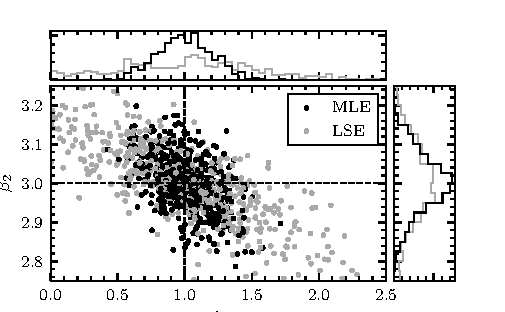
\includegraphics[width=10cm]{figures/toy_model_draws.pdf}
 	\caption{A repeated experiment followed by MLE and LSE estimation of the~parameters $\beta_1; \beta_2$, the~experiment as defined by Eqs.~\ref{eq:toy_model} - \ref{eq:toy_beta_values}. The~dashed lines show the~true value of $\vec{\beta}$. The~histograms of estimated $\beta_1$ and $\beta_2$ are shown in the~x-axis and y-axis histograms respectively.}
 	\label{fig:toy_model_draws}
\end{figure}

We note that the~presented fitting task is really relatively difficult, since majority of detections come from high $y_i$, where the~component $\propto y_i^5$ is very dominant compared to the~component $\propto y_i$, and it is easily seen in Fig.~\ref{fig:toy_model_draws} that it is the~$\beta_1$, which is estimated by LSE much more poorly than by MLE. The~information is however still there, since for low $y_i$, it is $\beta_1$, which is important. It turns out that LSE is too crude to yield the~information fully. We note that it is often the~case in practice, that Poission distributed data is fitted WLSE, assuming $\sigma_i = \sqrt{n_i}$ weights. This places more emphasis on the~lower values, but is only appropriate for the~values of $n_i$ high enough, so that $\sqrt{n_i} \ll n_i$, since $\sigma = \sqrt{\mu}$ for Poisson distribution, see Fig.~\ref{fig:pois_vs_norm}. This is quite incorrect for low values, and not viable at all for $n_i = 0$, as such a~weighting would incorrectly assume that all zeroes must have come out as a~result of the~rate $\Lambda = 0$, which is clearly not true, as seen in Fig.~\ref{fig:pois_vs_norm}. Sometimes weighting with $\sqrt{n_i+1}$ is used, in which $+1$ is a~rather arbitrary constant, and which is still not correct, and in our specific case is not even an unbiased estimate, as is demonstrated in Fig.~\ref{fig:toy_model_draws_weighted}. 

\begin{figure}[ht]
 	\centering
 	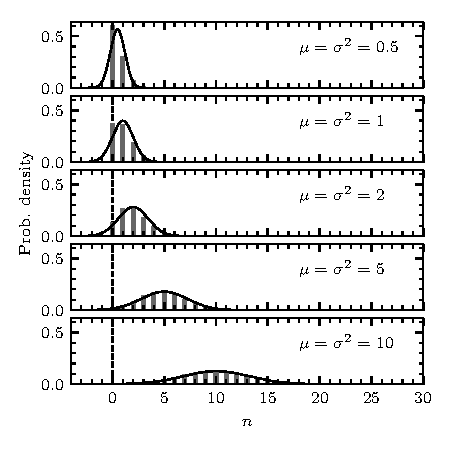
\includegraphics[width=10cm]{figures/pois_vs_norm.pdf}
 	\caption{A comparison of Poisson and normal distributions with identical mean $\mu$ and standard deviation $\sigma$.}
 	\label{fig:pois_vs_norm}
\end{figure}

\begin{figure}[ht]
 	\centering
 	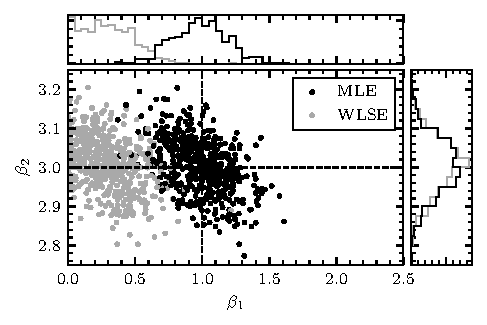
\includegraphics[width=10cm]{figures/toy_model_draws_weighted.pdf}
 	\caption{A repeated experiment followed by MLE and WLSE estimation of the~parameters $\beta_1; \beta_2$, the~experiment as defined by Eqs.~\ref{eq:toy_model} - \ref{eq:toy_beta_values}. The~weights in WLSE are $w_i = (1+n)^{-0.5}$, and the~WLSE is in this case not an unbiased estimate, since too much weight is put on the~$n_i=0$ data points. However, we observe that the~estimation of $\beta_2$ is not burdened by this, as the~WLSE points show even less variance in $\beta_2$, compared to LSE estimates in Fig.~\ref{fig:toy_model_draws}.}
 	\label{fig:toy_model_draws_weighted}
\end{figure}

Lastly, we note that the~presented toy model shares some characteristics with dust flux fitting. The~linear combination of several components as in Eq.~\ref{eq:linear_comination_model} is often assumed \citep{szalay2021collisional,zaslavsky2012interplanetary}, as we also did in Paper II. The~dust detection rate with spacecraft also often changes over several orders of magnitude, and is much lower if certain components are dominant, which might, similar to the~presented example, lead to a~bias, if not treated carefully. 

\section{Bayesian statistics}

Probability is a~complicated epistemological concept. Intuitively understood, probability becomes difficult, if confronted with other related concepts, such as causality, knowledge, or choice. In Bayesian statistics, unknown parameters are regarded as random variables, with their probability distribution representing the~state of knowledge or belief about them, and with data being used to improve the~level of this knowledge. a~event $A$ is regarded as having high probability, if it is reasonable to expect that the~event $A$ happens. This is put in contrast with so-called frequentist interpretation of probability, in which probability is regarded as the~long-term average frequency of the~event $A$ happening under the~same circumstances, as the~unknown parameters are treated as free, but not random variables. This doesn't make a~difference in many practical applications, but the~formulation of statistical task might be different. a~typical frequentist task is to assess the~most likely value (MLE) of an unknown (but certain) parameter, given what evidence was observed. If more data is considered, the~most likely value might change. In a~typical Bayesian task, a~probability density of the~value of the~unknown parameter is inferred, approaching the~unknown parameter as a~random variable. If more data is added, knowledge gets better, and the~probability distribution becomes narrower.

\subsection{Bayes theorem}

Bayes theorem stems from the~axiom of probability:
\begin{equation}
    P(A \cap B) = P(A|B)P(B) = P(B|A)P(A),
\end{equation}
which states that the~probability of events $A$ and $B$ occurring together is the~same as the~product of probabilities of one of them occurring, given the~other one does and the~other one occurring. The~Bayes theorem  \citep{bayes1763essay} in its modern form states:
\begin{equation}
    P(A|B) = \frac{P(B|A)P(A)}{P(B)},
    \label{eq:bayes_theorem}
\end{equation}
whenever $P(B) \neq 0$. This equation is instrumental to many statistical problems, such as evaluating blinded experiments, commonly used in medicine and other sciences. It also builds the~basis for Bayesian inference.

\subsection{Bayesian inference}

Assume a~model family $f_X$ is known, as well as the~data $\vec{x}$, which are realizations of the~random variable $X$. Similarly to Sec.~\ref{ch:mle}, we are interested in the~parameters $\vec{\theta}$. With MLE in Sec.~\ref{ch:mle}, the~goal was to find the~\textit{single value} $\vec{\theta}$, which fits the~data best, that is $\vec{\theta}$ with the~highest likelihood. However, MLE does not by itself provide any measure of uncertainty. 

Bayesian estimation needs a~\textit{prior distribution} of $\vec{\theta}$, denoted $\pi(\vec{\theta})$ to be defined on top of the~model family $f_X$ and the~data $\vec{x}$. This distribution represents our \textit{prior belief} in the~value of $\vec{\theta}$ before the~data $\vec{x}$ are examined. Described mathematically, we assume that $\vec{\theta}$ is a~random variable with the~value in the~space $\Theta$ coming from the~prior distribution $\pi(\vec{\theta}); \ \theta \in \Theta$. Without the~actual realization of $\vec{\theta}$ being known, this $\vec{\theta}$ plays the~role of a~parameter in $f_X(x|\vec{\theta})$, which generates the~sample of data $\vec{x}$, which is observed. Based on the~value of $\vec{x}$, which was observed, the~belief in $\theta$, represented by $\pi$, changes. The~goal is to obtain $\pi(\vec{\theta}|\vec{x})$, which not only provides the~most compatible value of $\vec{\theta}$, but also a~measure of uncertainty. 

The~desired posterior distribution $\pi(\vec{\theta}|\vec{x})$ is evaluated using the~Bayes theorem (Eq.~\ref{eq:bayes_theorem}):
\begin{equation}
    \pi(\vec{\theta}|\vec{x}) = \frac{p(\vec{x}|\vec{\theta}) \pi(\vec{\theta})}{p(\vec{x})} = \frac{\mathcal{L}(\vec{\theta}|\vec{x}) \pi(\vec{\theta})}{p(\vec{x})} \propto \mathcal{L}(\vec{\theta}|\vec{x}) \pi(\vec{\theta}),
    \label{eq:bayesian_inference}
\end{equation}
where the~equality becomes proportionality for practical reasons: it is often difficult to evaluate the~normalization factor $p(\vec{x})$, and if, for example, a~sampling procedure is used to evaluate the~right hand side, the~result is automatically normalized. 

For demonstration purposes, we apply Bayesian inference on the~problem defined by Eqs.~\ref{eq:toy_model} -- \ref{eq:toy_beta_values}. We use identical and independent priors for $\beta_1$ and $\beta_2$:
\begin{equation}
    \pi(\beta_i) = \sqrt{\frac{2}{\pi}} e^{\left(-\frac{\beta_i^2}{2}\right)} \mathbbm{1}_{\mathbb{R}^+} ,
\end{equation}
that is standard normal distribution for positive numbers, and zero elsewhere. We draw $150$ numbers $y_i$ from uniform distribution between zero and two, as before. For each $y_i$ we draw $n_i$ according to Eq.~\ref{eq:toy_model}. In Fig.~\ref{fig:bayesian_multivariate} we show the~MLE, LSE, and Bayesian results compared. Unlike in Fig.~\ref{fig:toy_model_draws}, the~experiment is done only once, therefore yielding only one MLE and one LSE estimate. In principle, Bayesian inference solves a~different task, compared to MLE. The~Bayesian posterior is not a~point, but a~multivariate distribution function, which, unlike the~other two estimates, shows a~measure of uncertainty. The~prior is consequential for Bayesian inference. However, the~prior becomes less important as the~number of data points increases. If data is plentiful and the~support of the~prior covers the~MLE estimate, the~maximum of Bayesian posterior (called \textit{maximum a~posteriori}, or MAP) is in practice equivalent to the~MLE estimate, as is demonstrated in Fig.~\ref{fig:bayesian_multivariate}, where the~relatively broad prior does not influence the~posterior much, compared to the~$150$ data points. We showed the~result of a~repeated experiment in Fig.~\ref{fig:toy_model_draws}. The~Bayesian posterior moves in a~repeated experiment, with the~actual values of $(\beta_1,\beta_2) = (1,3)$ likely being included in the~mass of the~posterior. Increasing the~number of data points beyond $150$ will then make the~posterior more localized with the~MAP closer to the~point $(1,3)$. To demonstrate this, we use the~same procedure to obtain the~posterior distribution for $\beta_1$ and $\beta_2$, but using a~gradually increasing number of points $y_i$ and corresponding $n_i$. We show the~maxima of the~posterior marginal distributions and symmetric $90 \, \%$ credible intervals as functions of the~number of drawn data points $n_i$. This is shown in Fig.~\ref{fig:bayesian_demosntration}.

\begin{figure}[ht]
 	\centering
 	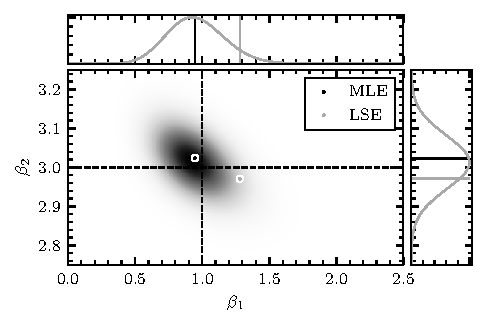
\includegraphics[width=10cm]{figures/bayesian_multivariate.pdf}
 	\caption{A comparison of the~Bayesian estimate and the~points estimates MLE and LSE, including $150$ data points. $\beta_1$ and $\beta_2$ marginal posteriors are shown in the~top and in the~right panel, with the~lines showing the~$MLE$ and $LSE$ estimates.}
 	\label{fig:bayesian_multivariate}
\end{figure}

\begin{figure}[ht]
 	\centering
 	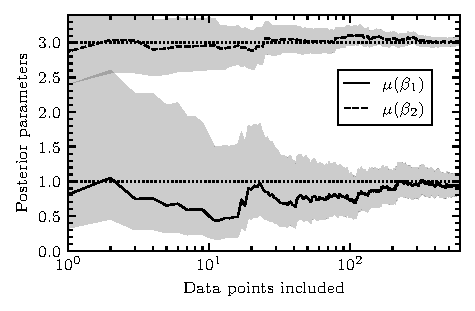
\includegraphics[width=10cm]{figures/bayesian.pdf}
 	\caption{A repeated experiment followed by Bayesian inference of the~parameters $\beta_1; \beta_2$, the~experiment as defined by Eqs.~\ref{eq:toy_model} - \ref{eq:toy_beta_values}. $\mu(\cdot)$ denotes the~posterior mean. The~shaded regions show symmetric $90 \, \%$ credible intervals. The~priors prefer values lower than the~actual $\beta_1=1;\,\beta_2=3$ but are broad and play a~small role once many data points are included. We note that $\beta_2$ is much better constrained, compared to $\beta_1$.}
 	\label{fig:bayesian_demosntration}
\end{figure}

\subsection{Computational methods}

\paragraph{Conjugate priors}
In special cases, the~task of inferring the~posterior distributions of the~unknown parameters might be approachable analytically, through so-called \textit{conjugate priors}. The~strongest requirement is that the~prior and the~likelihood are of certain families, for which analytical solutions were found. Many useful family combinations were described \citep{fink1997compendium}, as before the~boom in computational power, this was the~most practical way of doing Bayesian inference. All other methods described in further paragraphs of this section are numerical, that is, approximate.

\paragraph{Grid evaluation}
The~most straight-forward way of finding the~approximate posterior $\pi(\vec{\theta}|\vec{x})$ is to define a~grid in $\Theta$ and to evaluate the~product of the~likelihood and the~prior (Eq.~\ref{eq:bayesian_inference}) in all the~grid points. To maintain a~good resolution, the~number of grid points scales with the~power equal to the~dimension, hence, this approach easily becomes memory and time intensive. Furthermore, normalization might be difficult, and the~choice of grid points can be non-trivial. Many of these disadvantages are abated if a~sampling method is used instead. 

\paragraph{Markov chain Monte Carlo}
The~posterior $\pi(\vec{\theta}|\vec{x})$ can be approximately reconstructed and many of its features are available easily, if a~sample of values $\theta$ drawn from $\pi(\vec{\theta}|\vec{x})$ is available. This is the~idea of Markov chain Monte Carlo ({MCMC}) Bayesian inference. The~discrete Markov chain is a~stochastic process, in which the~current state is a~random value, probability of which is governed by the~preceding value \citep{markov1906extension}, forming a~random walk. If the~conditions of the~Markov chain central limit theorem are met \citep{jones2004markov}, this walk reaches a~stationary state, in which the~elements are distributed as if they were coming from a~distribution. Using the~right Markov chain, it is possible to draw a~sample from any probability density function. The~common methods of constructing the~appropriate Markov chain include \textit{Metropolis-Hastings} ({M-H}) algorithm, \citep{metropolis1953equation,hastings1970monte}, \textit{Gibbs sampling} \citep{geman1984stochastic}, and \textit{slice sampling} \citep{damlen1999gibbs}. These all have different strengths, and their computational efficiency varies based on the~problem at hand, but in higher dimensions, with a~more complicated model, or a~big data set, they are computationally expensive. Their common disadvantage is that, since the~samples form a~Markov chain, the~subsequent values are correlated. This usually does not pose an issue but must be kept in mind and handled carefully. MCMC remains popular, since it is very versatile and allows for evaluating virtually any Bayesian inference problem. Further introduction into MCMC is available in literature \citep{brooks2011handbook}. 

\paragraph{Integrated nested Laplace approximation}
Since MCMC is very versatile, but computationally expensive, and conjugate priors can only be used on a~narrow class of problems, a~method is needed which would be fairly generally useful, but computationally efficient. Integrated nested Laplace approximation ({INLA}) is one such a~method \citep{rue2009approximate,martins2013bayesian}, as it avoids sampling the~posterior distribution, and rather approximates the~posterior distributions analytically. It allows for fitting two-level, hierarchical models. On the~lower-level, the~parameters for the~higher-level distributions are contained. These lower-level parameters are called \textit{hyperparameters}, and they are random variables with priors called \textit{hyperpriors}, which are defined explicitly. On this lower-level, the~hyperparameters are used to construct the~higher-level parameters, called \textit{latent parameters}, which are used in the~higher-level distribution functions of the~observed data. This hierarchical setup is very convenient in spatio-temporal modelling, where the~data is often grouped in some way, as some of the~data points are close to each other, either in location or in time. It poses some limitations:
\begin{itemize}
    \item hyperparameters are assumed independent,
    \item the~number of hyper-parameters $n$ needs to be relatively low, that is $n \lesssim 10$,
    \item due to the~use of Laplace approximations, the~model must be \textit{latent Gaussian}, which means that the~latent parameter vector is assumed to come from a~multivariate Gaussian distribution.
\end{itemize}
Considering the~hierarchical form of INLA with observations $\vec{x}$, latent effects $\vec{z}$ and hyperparameters $\vec{\theta}$, and sticking with the~notations of probability rather than likelihood, Eq.~\ref{eq:bayesian_inference} has the~form \citep{gomez2020bayesian}:
\begin{equation}
    \pi(\vec{z}, \vec{\theta}|\vec{x}) \propto p(\vec{x}|\vec{z}, \vec{\theta}) p(\vec{z}|\vec{\theta}) \pi(\vec{\theta}).
    \label{eq:bayesian_hierarchical}
\end{equation}
Assuming the~independence of data $\vec{x}$ given $\vec{z}$ and $\vec{\theta}$, we get
\begin{equation}
    p(\vec{x}|\vec{z}, \vec{\theta}) \propto \prod_{i=1}^{k}p(x_i|y_i, \vec{\theta}),
\end{equation}
and since the~latent parameter vector $\vec{z}$ comes from the~multivariate Gaussian distribution, we have
\begin{equation}
    p(\vec{z}|\vec{\theta}) = |\tensor{Q}(\vec{\theta})|^{\frac{1}{2}} e^{-\frac{1}{2} \vec{z}^T \tensor{Q}(\vec{\theta}) \vec{z} },
\end{equation}
where $\tensor{Q}(\vec{\theta})$ is the~precision matrix of the~latent multivariate Gaussian distribution. Now by moving the~product to the~exponent, we get
\begin{equation}
    \pi(\vec{z}, \vec{\theta}|\vec{x}) \propto |\tensor{Q}(\vec{\theta})|^{\frac{1}{2}} e^{\left(-\frac{1}{2} \vec{z}^T \tensor{Q}(\vec{\theta}) \vec{z} + \sum_{i=1}^{k}\ln{p(x_i|y_i, \vec{\theta})} \right)} \pi(\vec{\theta}).
\end{equation}
The~goal of INLA is to obtain the~posterior marginals of the~unknown hyperparameters and the~latent parameters. For the~marginal of each of the~hyperparameters in $\vec{\theta}$ we get by definition
\begin{equation}
    \pi(\theta_j|\vec{x}) = \int_{\mathbb{R}^{n-1}}\pi(\vec{\theta}|\vec{x}) \, d\vec{\theta}_{-j}, 
\end{equation}
where $\vec{\theta}_{-j}$ stands for the~vector of all hyperparameters except for $\theta_j$. Similarly for the~latent parameters $\vec{z}$ we have
\begin{equation}
    \pi(z_i|\vec{x}) = \int_{\mathbb{R}^{n}} \pi(z_i|\vec{\theta},\vec{x}) \pi(\vec{\theta}|\vec{x}) \, d\vec{\theta}.
\end{equation}
The~previous equation is solved approximately on a~finite grid of $M$ hyperparameter values $\vec{\theta}_m$:
\begin{equation}
    \tilde{\pi}(z_i|\vec{x}) = \sum_{m=1}^M \tilde{\pi}(z_i|\vec{\theta}_m,\vec{x}) \tilde{\pi}(\vec{\theta}_m|\vec{x}) \Delta_m,
\end{equation}
where $\tilde{\pi}$ is an approximation of the~probability function $\pi$ and $\tilde{\pi}(z_i|\vec{\theta}_m,\vec{x})$ is approximated, for example with Laplace approximation. To evaluate both integrals, an approximation $\tilde{\pi}(\vec{\theta}|\vec{x})$ is needed. This is done as 
\begin{equation}
    \tilde{\pi}(\vec{\theta}|\vec{x}) \propto \frac{ \pi(\vec{x}|\vec{z},\vec{\theta}) \pi(\vec{z}|\vec{\theta}) \pi(\vec{\theta})}{\tilde{\pi}_G(\vec{z}|\vec{\theta},\vec{x})}|_{x=x^*},
\end{equation}
where $\tilde{\pi}_G(\vec{z}|\vec{\theta},\vec{x})$ is a~Gaussian approximation, which is justified, since the~latent effects $\vec{z}$ are Gaussian. The~INLA toolbox is available as a~library {R-INLA} \citep{rinla} and allows for convenient use via a~function call, including options for many popular hyperpriors, latent random effects, different approximations of $\tilde{\pi}(z_i|\vec{\theta} \vec{x})$, and a~lot of freedom for special purposes. Both the~background and a~practical user guide for R-INLA is offered in the~book by \citet{gomez2020bayesian}. To use R-INLA in a~simple Poisson case, such as in the~toy model defined by Eqs.~\ref{eq:toy_model} - \ref{eq:toy_beta_values}, a~vector of measured counts is needed, in addition to a~vector of covariates of same length, which would be the~$y_i$ and $y_i^5$ values in this specific case. In Paper II. of this thesis, we used INLA to fit dust rates observed by SolO in a~similar setup, where the~higher-level was degenerate, and only the~hyperparameters were used in a~nonlinear rate-defining model, making use of INLA's speed, although not utilizing its spatial modelling potential. 

\subsection{The~importance of prior}

The~prior distribution $\pi(\vec{\theta})$ represents the~prior belief about the~value of $\vec{\theta}$ and it might be based for example on previous estimations, personal preference, community consensus, or computational convenience, and each of these choices might lead to a~different result and implies a~different meaning of the~result. This is why the~necessity of prior is often regarded as a~disadvantage of the~Bayesian approach. On the~other hand, inclusion of the~prior makes the~process more transparent. a~non-Bayesian parameter estimation is often followed by a~discussion comparing the~result with previous estimates and discussing the~limits of applicability. Alternatively, the~result might not get published, if it doesn't match the~expectations. The~expectations and other constraints could be transparently included in the~form of a~prior.

\paragraph{Non-informative prior} a~flat prior ($\pi = const.$) is often used and assumed to be a~neutral starting point. In such a~case, the~likelihood is effectively treated as being the~posterior distribution, except for the~normalization prefactor. Although the~flat prior can be a~legitimate choice, it is important to appreciate that any prior choice is a~choice, and there is no prior without assumptions. Flat prior implies that all the~possible values of the~inferred parameter are equally possible and expected, which is untruth more often than not. Furthermore, depending on the~model, domain, data, coordinates, and the~transformation used, flat prior might not be the~least informative \citep{lemoine2019moving}.

Another aspect of flat priors is that a~flat prior over $\mathbb{R}$ is not a~valid probability density function. Therefore, a~flat prior over a~great finite range is often used, with zero probability elsewhere. Depending on the~numerical method, an \textit{improper prior} might be used, which is a~non-integrable prior, provided that the~likelihood factor $\mathcal{L}(\vec{\theta}|\vec{x})$ ensures the~integrability of the~results. The~interpretation of such a~result is complicated, as the~assumptions of the~Bayes theorem are not met. 

Conversely, the~likelihood factor might be non-integrable, which is not an issue, if both the~prior and the~posterior are. This is often the~case when a~single data point is used to get the~posterior. In such a~case, the~choice of prior is very consequential. Generally speaking, the~importance of prior is the~lower, the~more data points are used to construct the~likelihood.

\paragraph{Informative prior} Using a~non-flat, \textit{weakly informative} prior might be numerically beneficial by ensuring integrability of the~posterior. Also, extrema are relatively rare in higher dimension. For a~stationary point to be an extremum rather than a~saddle point, the~sign of the~second derivative must be the~same in all the~dimensions, which is automatically satisfied in one dimension, but rarely satisfied in high dimensions. Multiplying the~likelihood with an appropriate (weakly informative) prior might make this problem numerically a~lot easier. 

Existing knowledge might be leveraged, when constructing a~prior. We then speak of \textit{informative} prior, as it holds a~non-trivial information. Such a~prior must be backed by theory rather than to be constructed based on the~inspection of the~available data, otherwise the~same information is harnessed twice. These are especially useful if only a~few data points are available. In Paper II, we used moderately informative priors. We could do so, since the~unknown parameters were constrained by previous results of other authors and by physics, as not all the~values were physically meaningful. 







